\section{Engine}
\label{verwendung_engine}
Wenn sie die FM3D-Engine in Kombination mit dem FM3D-Designer verwenden, so wird Ihnen bei der Projekterstellung ein funktionsfähiges VisualStudio C++ Projekt generiert, welches in der VisualStudio-Solution \textit{GameProject.sln} zu finden ist.
Es wird ihnen geraten, nichts an dem generierten Code zu ändern.
In der Datei \textit{"'presets.h"`} werden die Entity-Presets generiert, welche Sie im Designer erstellen können.
Sie können dem Projekt auch neue Dateien hinzufügen und unabhängig vom generierten Code programmieren. Weitere Dateien, welche ursprünglich nicht zu dem generierten Projekt gehört haben sollten keinen Einfluss auf die Funktionalität des generierten Codes haben.
Das Spiel an sich steht in der Main.cpp Datei, welche im Projekt bereits vorhanden ist.

\subsection{Voreinstellungen}
Zunächst müssen sie die Bibliotheken der FM3D-Engine, OpenGL, FreeImage, FreeType und Assimp in das Projekt einbinden. Falls Sie die Engine in Kombination mit dem FM3D-Designer verwenden, so werden die Verzeichnisse automatisch eingebunden. Falls nicht, so müssen Sie die Verzeichnisse manuell einbinden. Fügen Sie die Verzeichnisse in die zugehörige Option hinzu. Das ganze sollte so in ihren Einstellungen aussehen:
$$Configuration Properties->C/C++->Additional Include Directories$$\cref{includeinc}
$$Configuration Properties->Linker->Additional Include Directories$$
\cref{liblib}

\begin{figure}
	\begin{center}
		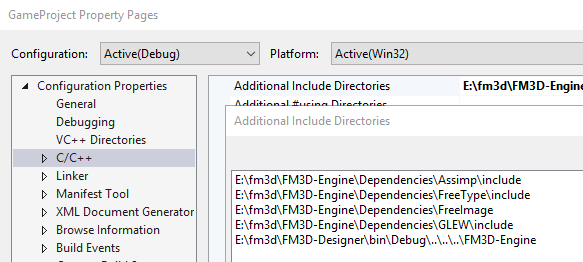
\includegraphics[width=\textwidth]{04verwendung/Engine/include.png}
		\caption{Include Verzeichnisse}\label{includeinc}
	\end{center}
\end{figure}

\begin{figure}
	\begin{center}
		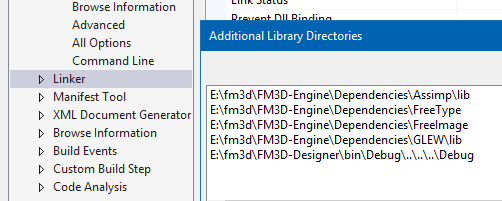
\includegraphics[width=\textwidth]{04verwendung/Engine/lib.png}
		\caption{Lib-Verzeichnisse}\label{liblib}
	\end{center}
\end{figure}

\subsection{Kamera}
Die Kamera ist in dem Generierten Projekt bereits vorhanden. Ihnen wird empfohlen die Werte der Position, Rotation und Zoom der Kamera im Bereich der \textit{Game-Logic} zu verändern. Auch dieser Bereich ist eindeutig mit Kommentaren kenntlich gemacht. Für Infos über den Syntax der Kamera wird empfohlen in der DoxyGen-Dokumentation die Klasse "`Camera"' nachzuschlagen.

\subsection{Entities}
Erstellen Sie zunächst die Entities an der eindeutig kommentierten Stelle \textit{"'Create Entities here"`}. Erstellen Sie zunächst beliebig viele Preset-Objekte ihrer erstellten Entity-Preset-Klasse. Sie können nun bei jedem beliebigen Objekt "`Preset-Einstellungen"' tätigen, in dem Sie dem Entity-Preset-Objekt Standardwerte zuweisen. 
Initialisieren Sie nun einen Entity-Pointer (Klasse: \textit{EntityPtr}) und erstellen sie das Entity in der bereits initialisierten \textit{EntityCollection} namens \textit{scene}. Als Beispiel:
\begin{lstlisting}{Entity}
EntityCollection scene;
EntityPtr baum = scene.CreateEntity();
\end{lstlisting}
Diese beinhaltet alle Entities die in dem Spiel verwendet werden.
%Beispiel
Wenn ein Entity das Komponent \textit{RenderableComponent} besitzt, so kann es in dem eindeutig kommentierten Abschnitt "'Submit objects here to renderer"` dem Renderer übergeben werden.
%Beispiel
Bevor Sie den Entities die Modelle zuweisen, vergessen Sie nicht die Modelle in die Projektmappe von VisualStudio zu laden.

\subsection{Inputsystem}
\label{inputsystemver}
Hierfür wird die Klasse \textit{Input} verwendet. Möchte man nun Tasten abfragen, so muss man zunächst über das Fenster auf das Objekt der Klasse Input zugreifen. 
Nun kann eine Methode aus dieser Klasse verwendet werden.
Möchten Sie nun abfragen, ob zB. die Taste F5 auf der Tastatur gedrückt wurde, so schreiben Sie dies so in den Code:
\begin{lstlisting}{Input}
win->GetInput().CheckKey(KEY_F5);
\end{lstlisting}
Möchten Sie nun überprüfen ob die Linke Maustaste gedrückt wurde so tun Sie dies folgendermaßen:
\begin{lstlisting}{Input}
win->GetInput().CheckMouse(MOUSE_LEFT);
\end{lstlisting}

Möchte man nun die Position des letzten Klicks mit der linken Maustaste ermitteln, benutzt man diese Methode:
\begin{lstlisting}{Input}
win->GetInput().GetLastposClick(MOUSE_LEFT);
\end{lstlisting}
Diese gibt einen zweidimensionalen Vektor vom Typ Float zurück, welcher die Position vom letzten Klick der Maus mit einer bestimmten Maustaste beschreibt. 
Die folgende Methode gibt Daten in Form eines zweidimensionalen Vektors mit der aktuellen Position der Maus zurück.
\begin{lstlisting}{Input}
win->GetInput().GetLastposInst();
\end{lstlisting}

Alle Tasten der Tastatur und Maus können über Makros angesprochen werden. Auch können Sie die ASCII-Codes der einzelnen Tasten verwenden. Die Makros, welche die Tasten der Tastatur beschreiben starten mit \textit{"`KEY\_"'}. Die Makros, die für die Maus verwendet werden starten mit \textit{"`MAUS\_"'}.
